\subsection{Adding a layer}
\label{subsection:experiments:classification:adding-a-layer}
In this subsection, we will focus on neural networks with two hidden layers of the same width. The experiment configuration is almost identical to one from the previous section. The only change is the addition of another identical hidden layer to each neural network.
For each experiment configuration, the model achieving the best validation accuracy is saved and used in the following analysis.

From Figure \ref{fig:experiments:classification:all-activations-plot}, it is noticeable that the best validation accuracy increases consistently with the hidden layer width. This may suggest that $\operatorname{sigmoid}$ and $\operatorname{tanh}$ neural networks may benefit from the increased model complexity. However, it seems that this does not happen to the extent one may expect (see Figure \ref{fig:experiments:classification:adding-a-layer-all-activations}).

In the previous section, we discussed the similarity between the $\operatorname{sigmoid}$ and $\operatorname{tanh}$ activation function. From the Figure \ref{fig:experiments:classification:adding-a-layer-all-activations}, we can conclude that $\operatorname{sigmoid}$ and $\operatorname{tanh}$ networks remain achieving similar validation accuracy, what is compatible with results from the previous section.

From Figure \ref{fig:experiments:classification:adding-a-layer-sigmoid}, Figure \ref{fig:experiments:classification:adding-a-layer-tanh} and Figure \ref{fig:experiments:classification:adding-a-layer-relu}, it is evident that the layer addition results in slightly better validation accuracy for layer widths up to and including 128 neurons. However, the difference is mostly within $1.5\%$ and this can be attributed to the noise. It is hard to say whether the validation accuracy boost is significant. According to the benchmark table in \cite{fashionmnistgithub}, similar neural networks may achieve the validation accuracy of $88\%$ (see the entry for \textit{MLP 256-128-100}). The pattern is slightly unclear for layer widths larger than 128 neurons. For instance, the network with $\operatorname{tanh}$ activation and two hidden layers of 512 neurons achieved the validation accuracy of $82.33\%$, which is the best validation accuracy so far. However, such a configuration performed noticeably less well for other activation functions, especially $\operatorname{ReLU}$.

Neural networks with $\operatorname{tanh}$ activation function benefited the most from the extra layer. According to Figure \ref{fig:experiments:classification:adding-a-layer-tanh}, $\operatorname{tanh}$ neural networks with two identical layers consistently performed at least as well as the corresponding single layer configuration. It is interesting to note that $\operatorname{ReLU}$ networks benefited the least from the extra layer. This observation is quite evident from the Figure \ref{fig:experiments:classification:adding-a-layer-relu}. As in the case of neural networks with the single layer, $\operatorname{ReLU}$ networks seem to generalize slightly worse than $\operatorname{tanh}$ and $\operatorname{sigmoid}$ networks.

\begin{figure}[H]
    \centering
    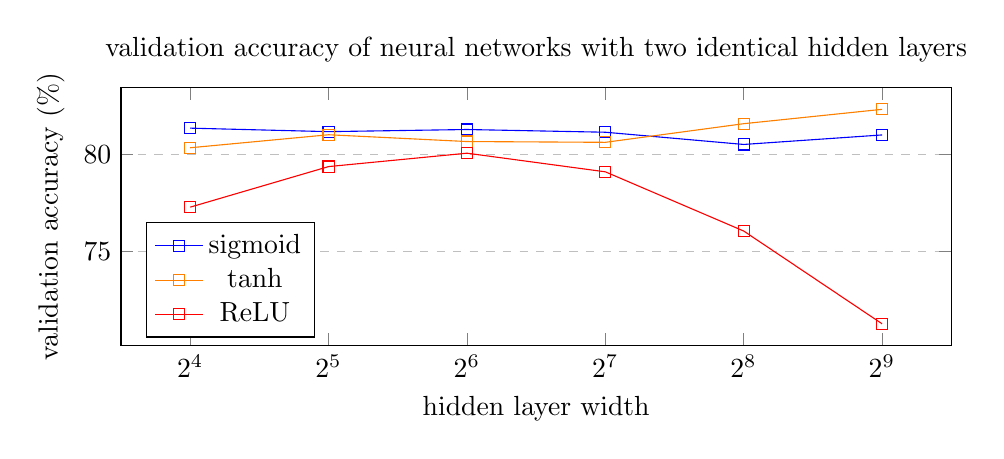
\begin{tikzpicture}
        \begin{axis}[
            height=0.4\textwidth,
            title={validation accuracy of neural networks with two identical hidden layers},
            width=\textwidth,
            xlabel={hidden layer width},
            ylabel={validation accuracy (\%)},
            ymajorgrids=true,
            grid style=dashed,
            xmode=log,
            legend pos=south west,
            log basis x={2}]
            \addplot[mark=square,blue] coordinates {(16,81.36) (32,81.18) (64, 81.29) (128,81.15) (256,80.52) (512,81.01)};
            \addplot[mark=square,orange] coordinates {(16,80.35) (32,81.02) (64,80.67) (128,80.63) (256,81.59) (512,82.33)};
            \addplot[mark=square,red] coordinates {(16,77.29) (32,79.38) (64,80.07) (128,79.11) (256,76.06) (512,71.28)};
            \legend{sigmoid, tanh, ReLU}
        \end{axis}
    \end{tikzpicture}
    \caption{Validation accuracy for networks with two identical hidden layers}
    \label{fig:experiments:classification:adding-a-layer-all-activations}
\end{figure}
\newpage
\begin{figure}[H]
    \centering
    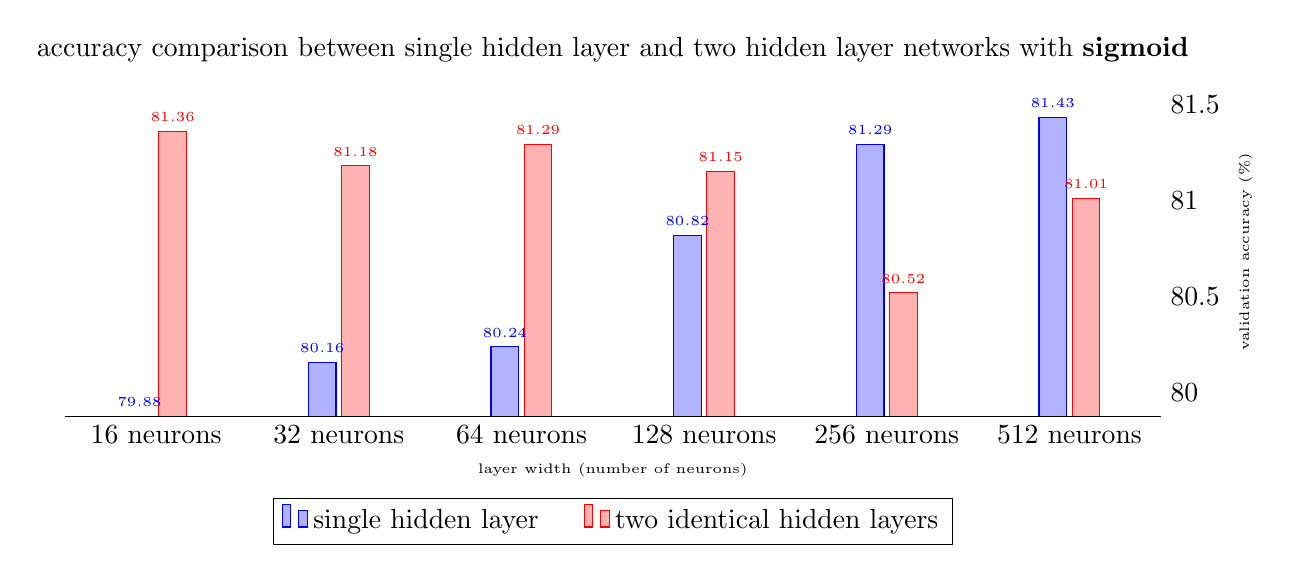
\begin{tikzpicture}
      \centering
      \begin{axis}[
            ybar, axis on top,
            title={accuracy comparison between single hidden layer and two hidden layer networks with \textbf{sigmoid}},
            height=5.75cm, width=15.5cm,
            tick align=inside,
            enlarge y limits={value=.1,upper},
            axis x line*=bottom,
            axis y line*=right,
            y axis line style={opacity=0},
            tickwidth=0pt,
            enlarge x limits=true,
            legend style={
                at={(0.5,-0.25)},
                anchor=north,
                legend columns=-1,
                /tikz/every even column/.append style={column sep=0.5cm}
           },
           ylabel={validation accuracy (\%)},
           symbolic x coords={
               16 neurons, 32 neurons, 64 neurons, 128 neurons,
               256 neurons, 512 neurons
           },
           xtick=data,
           xlabel={layer width (number of neurons)},
           label style={font=\tiny},
           every node near coord/.append style={font=\tiny},
           nodes near coords={
            \pgfmathprintnumber[precision=2]{\pgfplotspointmeta}
           }
        ]
        \addplot coordinates {
            (16 neurons,79.88) 
            (32 neurons,80.16) 
            (64 neurons,80.24) 
            (128 neurons,80.82) 
            (256 neurons,81.29) 
            (512 neurons,81.43)
        };
        \addplot coordinates {
            (16 neurons,81.36) 
            (32 neurons,81.18) 
            (64 neurons, 81.29) 
            (128 neurons,81.15) 
            (256 neurons,80.52) 
            (512 neurons,81.01)
        };
        \legend{single hidden layer, two identical hidden layers}
      \end{axis}
    \end{tikzpicture}
    \caption{Validation accuracy for \textbf{sigmoid}  grouped by number of layers}
    \label{fig:experiments:classification:adding-a-layer-sigmoid}
\end{figure}
\begin{figure}[H]
    \centering
    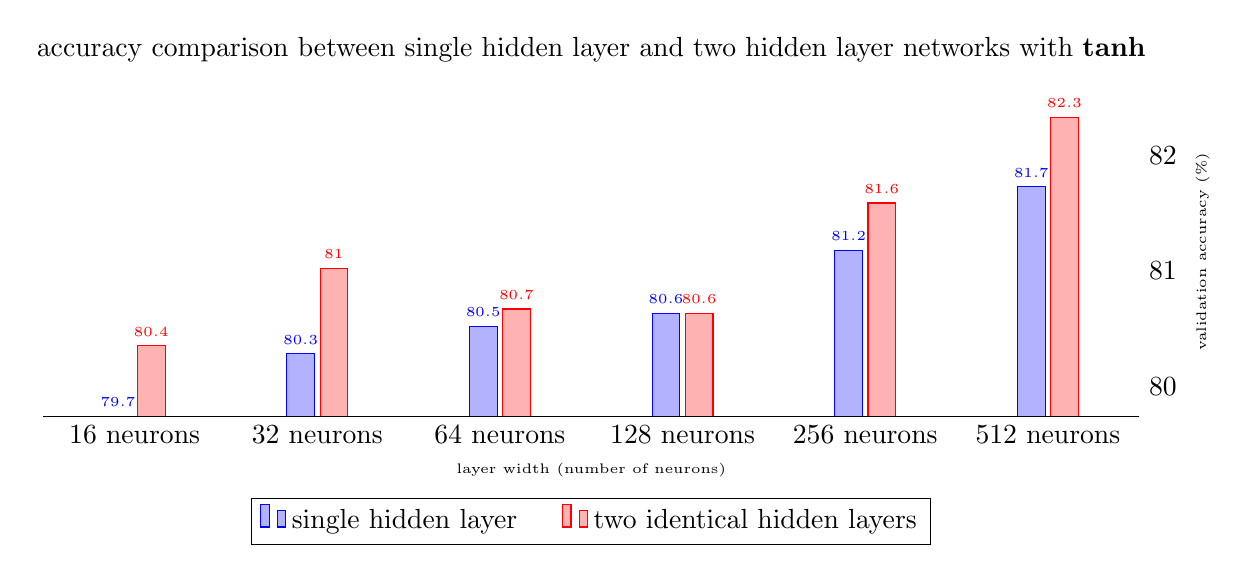
\begin{tikzpicture}
      \centering
      \begin{axis}[
            ybar, axis on top,
            title={accuracy comparison between single hidden layer and two hidden layer networks with \textbf{tanh}},
            height=5.75cm, width=15.5cm,
            tick align=inside,
            enlarge y limits={value=.1,upper},
            axis x line*=bottom,
            axis y line*=right,
            y axis line style={opacity=0},
            tickwidth=0pt,
            enlarge x limits=true,
            legend style={
                at={(0.5,-0.25)},
                anchor=north,
                legend columns=-1,
                /tikz/every even column/.append style={column sep=0.5cm}
           },
           ylabel={validation accuracy (\%)},
            symbolic x coords={
               16 neurons, 32 neurons, 64 neurons, 128 neurons,
               256 neurons, 512 neurons
            },
           xtick=data,
           xlabel={layer width (number of neurons)},
           label style={font=\tiny},
           every node near coord/.append style={font=\tiny},
           nodes near coords={
            \pgfmathprintnumber[precision=1]{\pgfplotspointmeta}
           }
        ]
        
        \addplot coordinates {
            (16 neurons,79.74) 
            (32 neurons,80.28) 
            (64 neurons,80.52) 
            (128 neurons,80.63) 
            (256 neurons,81.18) 
            (512 neurons,81.73)
        };
        \addplot coordinates {
            (16 neurons,80.35) 
            (32 neurons,81.02) 
            (64 neurons,80.67) 
            (128 neurons,80.63) 
            (256 neurons,81.59) 
            (512 neurons,82.33)
        };
        \legend{single hidden layer, two identical hidden layers}
      \end{axis}
    \end{tikzpicture}  
    \caption{Validation accuracy for \textbf{tanh} grouped by the number of layers}
    \label{fig:experiments:classification:adding-a-layer-tanh}
\end{figure}
\begin{figure}[H]
    \centering
    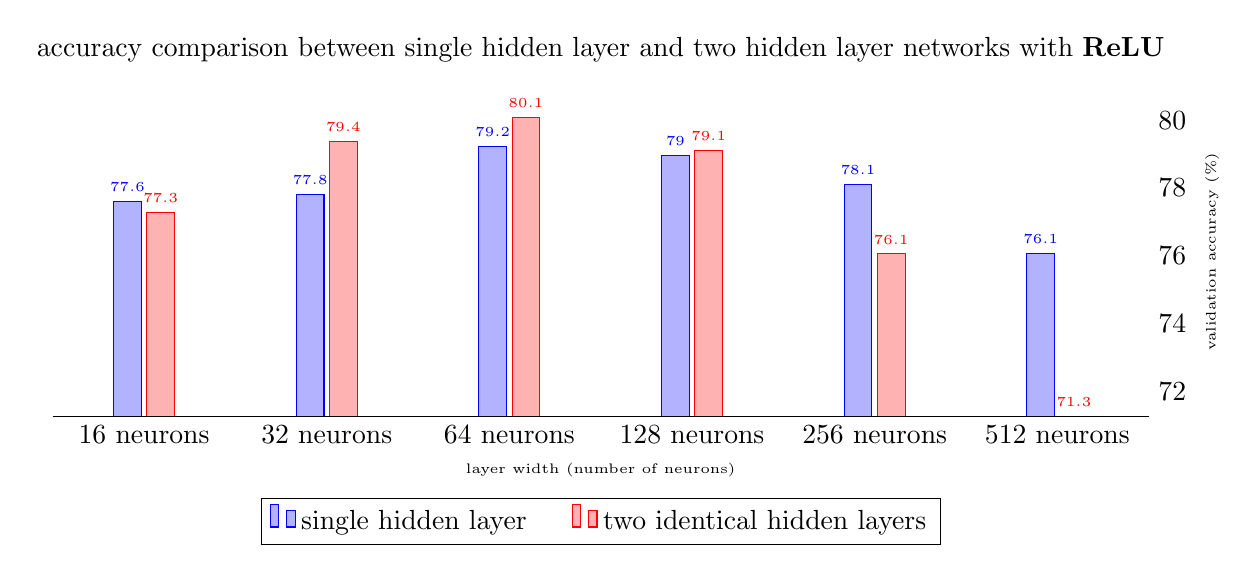
\begin{tikzpicture}
      \centering
      \begin{axis}[
            ybar, axis on top,
            title={accuracy comparison between single hidden layer and two hidden layer networks with \textbf{ReLU}},
            height=5.75cm, width=15.5cm,
            tick align=inside,
            enlarge y limits={value=.1,upper},
            axis x line*=bottom,
            axis y line*=right,
            y axis line style={opacity=0},
            tickwidth=0pt,
            enlarge x limits=true,
            legend style={
                at={(0.5,-0.25)},
                anchor=north,
                legend columns=-1,
                /tikz/every even column/.append style={column sep=0.5cm}
           },
           ylabel={validation accuracy (\%)},
            symbolic x coords={
               16 neurons, 32 neurons, 64 neurons, 128 neurons,
               256 neurons, 512 neurons
            },
           xtick=data,
           label style={font=\tiny},
           xlabel={layer width (number of neurons)},
           every node near coord/.append style={font=\tiny},
           nodes near coords={
            \pgfmathprintnumber[precision=1]{\pgfplotspointmeta}
           }
        ]
        \addplot coordinates {
            (16 neurons,77.60)
            (32 neurons,77.82) 
            (64 neurons,79.23) 
            (128 neurons,78.97) 
            (256 neurons,78.10) 
            (512 neurons,76.08)
        };
        \addplot coordinates {
            (16 neurons,77.29) 
            (32 neurons,79.38) 
            (64 neurons,80.07) 
            (128 neurons,79.11) 
            (256 neurons,76.06) 
            (512 neurons,71.28)
        };
        \legend{single hidden layer, two identical hidden layers}
      \end{axis}
    \end{tikzpicture}  
    \caption{Validation accuracy for \textbf{ReLU} grouped by the number of layers}
    \label{fig:experiments:classification:adding-a-layer-relu}
\end{figure}